\documentclass{standalone}
\usepackage{tikz,bm}
\begin{document}
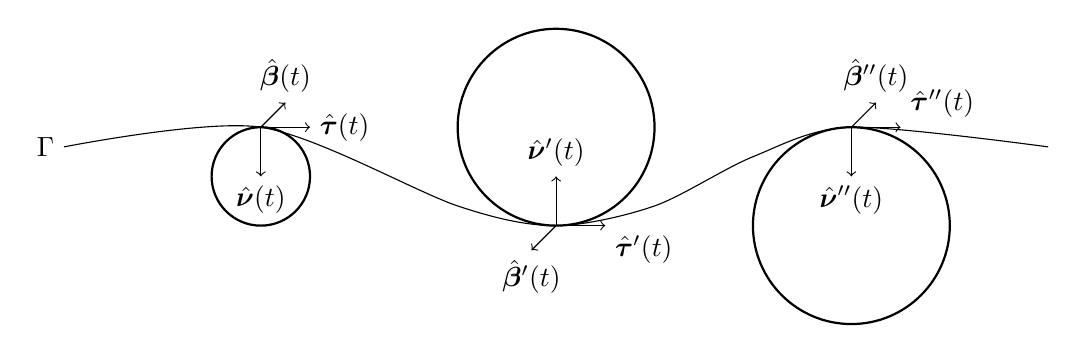
\begin{tikzpicture}[scale=1.25]
    \draw[thick](-2,-0.5)circle(0.5);
    \draw[thick](1,0)circle(1);
    \draw[thick](4,-1)circle(1);
    
    \node[left]at(-4,-0.2){$\Gamma$};
    \draw[-]plot[smooth]coordinates{(-4,-0.2)(-2,0)(0,-.8)(1,-1)(2,-0.8)(3,-0.3)(4,0)(6,-0.2)};

    \draw[->](-2,0)--(-1.5,0) node[right]{$\hat{\boldsymbol{\tau}}(t)$};
    \draw[->](-2,0)--(-1.75,0.25)node[above]{$\hat{\boldsymbol{\beta}}(t)$};
    \draw[->](-2,0)--(-2,-0.5)node[below]{$\hat{\boldsymbol{\nu}}(t)$};

    \draw[->](1,-1)--(1.5,-1) node[below right]{$\hat{\boldsymbol{\tau}}'(t)$};
    \draw[->](1,-1)--(0.75,-1.25)node[below]{$\hat{\boldsymbol{\beta}}'(t)$};
    \draw[->](1,-1)--(1,-0.5)node[above]{$\hat{\boldsymbol{\nu}}'(t)$};

    \draw[->](4,0)--(4.5,0) node[above right]{$\hat{\boldsymbol{\tau}}''(t)$};
    \draw[->](4,0)--(4.25,0.25)node[above]{$\hat{\boldsymbol{\beta}}''(t)$};
    \draw[->](4,0)--(4,-0.5)node[below]{$\hat{\boldsymbol{\nu}}''(t)$};
\end{tikzpicture}
\end{document}